% This file was created with tikzplotlib v0.10.1.
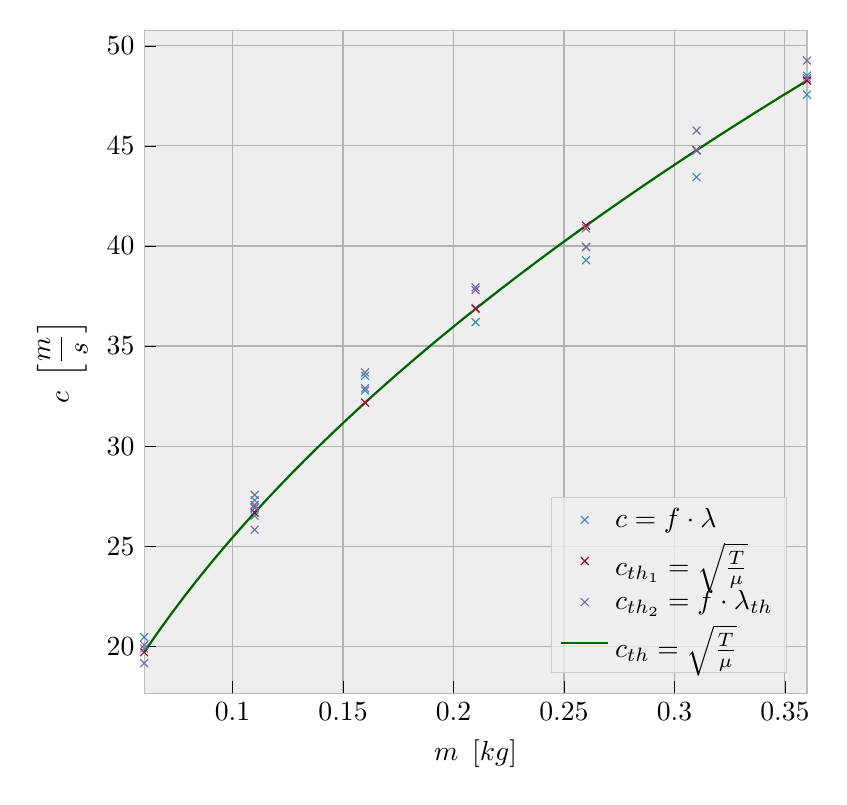
\begin{tikzpicture}

\definecolor{darkgray178}{RGB}{178,178,178}
\definecolor{darkgreen}{RGB}{0,100,0}
\definecolor{firebrick166640}{RGB}{166,6,40}
\definecolor{lightgray204}{RGB}{204,204,204}
\definecolor{silver188}{RGB}{188,188,188}
\definecolor{slategray122104166}{RGB}{122,104,166}
\definecolor{steelblue52138189}{RGB}{52,138,189}
\definecolor{whitesmoke238}{RGB}{238,238,238}

\begin{axis}[
axis background/.style={fill=whitesmoke238},
axis line style={silver188},
height=10cm,
legend cell align={left},
legend style={
  fill opacity=0.8,
  draw opacity=1,
  text opacity=1,
  at={(0.97,0.03)},
  anchor=south east,
  draw=lightgray204,
  fill=whitesmoke238
},
tick pos=left,
width=10cm,
x grid style={darkgray178},
xlabel={\(\displaystyle m \ \left[kg\right]\)},
xmajorgrids,
xmin=0.06, xmax=0.36,
xtick style={color=black},
y grid style={darkgray178},
ylabel={\(\displaystyle c \ \left[\frac{m}{s}\right]\)},
ymajorgrids,
ymin=17.6528, ymax=50.7703428571429,
ytick style={color=black}
]
\addplot [draw=steelblue52138189, fill=steelblue52138189, mark=x, only marks]
table{%
x  y
0.11 26.9335
0.11 27.2935
0.11 26.5226
0.11 26.9088
0.0600000000000001 19.89
0.0600000000000001 20.457
0.16 33.51183
0.16 32.7768
0.21 36.1939
0.21 36.9
0.26 39.9489
0.26 39.285
0.31 44.781
0.31 43.44
0.36 47.56
0.36 48.5135
};
\addlegendentry{$c = f \cdot \lambda$}
\addplot [draw=firebrick166640, fill=firebrick166640, mark=x, only marks]
table{%
x  y
0.11 26.6770772387081
0.0600000000000001 19.7023272737004
0.16 32.173765710591
0.21 36.8596791901395
0.26 41.0136647960165
0.31 44.7839865353678
0.36 48.2606485658865
0.36 48.2606485658865
};
\addlegendentry{$c_{th_1} = \sqrt{\frac{T}{\mu}}$}
\addplot [draw=slategray122104166, fill=slategray122104166, mark=x, only marks]
table{%
x  y
0.11 26.9335
0.11 27.0641428571429
0.11 25.8223333333333
0.11 27.5628333333333
0.0600000000000001 20.06
0.0600000000000001 19.1581428571429
0.16 33.6831
0.16 32.8882857142857
0.21 37.7954
0.21 37.9285714285714
0.26 39.9489
0.26 40.8785714285714
0.31 44.781
0.31 45.7671428571429
0.36 48.38
0.36 49.265
};
\addlegendentry{$c_{th_2} = f \cdot \lambda_{th}$}
\addplot [thick, darkgreen]
table {%
0.059999942779541 19.7023277282715
0.0660605430603027 20.6734600067139
0.072121262550354 21.6009769439697
0.0781818628311157 22.4902763366699
0.0842424631118774 23.345724105835
0.0903030633926392 24.1709136962891
0.0963636636734009 24.9688472747803
0.102424263954163 25.7420597076416
0.108484864234924 26.4927139282227
0.114545464515686 27.222677230835
0.120606064796448 27.9335708618164
0.126666665077209 28.6268177032471
0.132727265357971 29.3036689758301
0.138787865638733 29.9652347564697
0.144848465919495 30.6125049591064
0.150909066200256 31.2463722229004
0.156969666481018 31.8676338195801
0.16303026676178 32.4770126342773
0.169090867042542 33.0751647949219
0.175151467323303 33.6626930236816
0.184242486953735 34.5252418518066
0.193333387374878 35.3667602539062
0.202424287796021 36.1887168884277
0.211515188217163 36.9924125671387
0.220606088638306 37.7790145874023
0.229696989059448 38.5495681762695
0.238787889480591 39.3050231933594
0.247878789901733 40.0462265014648
0.256969690322876 40.7739562988281
0.266060590744019 41.4889259338379
0.275151491165161 42.191780090332
0.284242391586304 42.8831176757812
0.293333292007446 43.5634841918945
0.302424192428589 44.2333869934082
0.311515092849731 44.8932952880859
0.320605993270874 45.543643951416
0.329697012901306 46.1848335266113
0.338787913322449 46.8172416687012
0.347878813743591 47.4412231445312
0.360000014305115 48.2606468200684
};
\addlegendentry{$c_{th} = \sqrt{\frac{T}{\mu}}$}
\end{axis}

\end{tikzpicture}
